% Package loading etc.
%%%%%%%%%%%%%%%%%%%%%%%%%%%%%%%%%%%%%%%%%%%
\documentclass[10pt]{report}
\usepackage[margin=1.3in]{geometry}
\usepackage[utf8]{inputenc}
\usepackage{geometry}  
\usepackage{pifont}
\usepackage{subcaption}
\usepackage{booktabs}% See geometry.pdf to learn the layout options. There are lots.
\geometry{letterpaper}                   % ... or a4paper or a5paper or ... 
%\geometry{landscape}                % Activate for for rotated page geometry
\usepackage[parfill]{parskip}    % Activate to begin paragraphs with an empty line rather than an indent
\usepackage{graphicx}
\usepackage{amssymb, amsmath}
\usepackage{epstopdf}
\usepackage{float}
\usepackage{hyperref}
\usepackage{listings}
\usepackage{tabularx}
\usepackage{fancyhdr}
\usepackage{comment}
\usepackage{tcolorbox}
\usepackage{bm}
\usepackage{bbm}
\usepackage{tikz}
\usetikzlibrary{fit}

\tikzset{every label/.style={font=\footnotesize,inner sep=1.5pt}}

\newcommand{\stencilpt}[4][]{\node[circle,fill=blue,draw=blue, label={[shift={(-0.4,-0.0)}]below:#4},#1] at (#2) (#3) {}}
\usepackage{pifont}
\newtheorem{theorem}{Theorem}
\usetikzlibrary{automata,positioning}
\newcommand{\bigO}{\mathcal{O}}
\newcommand{\dd}[1]{\mathrm{d}#1}
\newcommand{\td}{\tilde}
\newcommand{\dx}{\Delta x}
\newcommand{\dt}{\Delta t}
\DeclareMathOperator{\Exp}{\text{Exp}}
\DeclareMathOperator*{\E}{\mathbb{E}}
\DeclareGraphicsRule{.tif}{png}{.png}{`convert #1 `dirname #1`/`basename #1 .tif`.png}
%%%%%%%%%%%%%%%%%%%%%%%%%%%%%%%%%%%%%%%%%%%%%


\title{\huge{Computational Fluid Dynamics}\\\Large{SG2212 Project Report}}
\author{\LARGE{David Ahnlund}}
\date{}


\begin{document}

\maketitle
\newpage% or \cleardoublepage
\pagestyle{fancy}
\fancyhead[L]{David Ahnlund}
\fancyhead[R]{SG2212 Project}
\fancyhead[C]{Lid-driven cavity}
%%%% Write from here:

\subsection*{Question 1}
The kronecker operator (\textbf{kron}) is an operator for tensor product, which falls convinient
when doing finite differences in higher dimensions than the 1D case. As we study the 2D case in this
lid-driven cavity project the 5 point stencil is considered:


\begin{figure}[h]
    \centering
    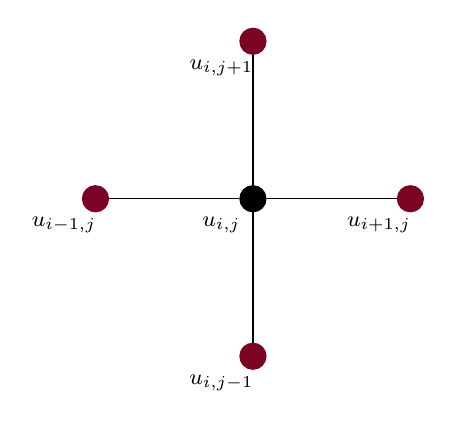
\begin{tikzpicture}[scale = 2]
        \definecolor{wine}{RGB}{123,3,35}
        \stencilpt[wine]{-1,0}{i-1}{$u_{i-1,j}$};
        \stencilpt[black]{ 0,0}{i}  {$u_{i,j}$};
        \stencilpt[wine]{ 1,0}{i+1}{$u_{i+1,j}$};
        \stencilpt[wine]{0,-1}{j-1}{$u_{i,j-1}$};
        \stencilpt[wine]{0, 1}{j+1}{$u_{i,j+1}$};
        \draw
        (i-1) -- (i)
        (i) -- (i+1)
        (i) -- (j+1)
        (j-1) -- (i);

    \end{tikzpicture}
    
    \caption{The five point stencil in 2D.} 
    \label{fivepoint}  
\end{figure}
If we construct a finite difference scheme for the laplace operator we get:
\begin{gather}
    \nabla^2u = \frac{u_{i+1,j}-2u_{i,j}+u_{i-1,j}}{h_x^2} + \frac{u_{i,j+1}-2u_{i,j}+u_{i,j-1}}{h_y^2}\\
    \left\{  \text{and if }h_x = h_y = h \implies \frac{u_{i+1,j}+u_{i-1,j} -4u_{i,j}+ u_{i,j+1}+u_{i,j-1}}{h^2} \right\}
    \label{simplelap}
\end{gather}
The above expression we can transform into a vector form in size $(N_x, N_y) \mapsto N_x \cdot N_y$, using the indexing
that one step in $y$-direction is equivalent to one row in the matrix \textit{i.e.} $+N_x$ steps.

We can now define the second partial derivative in the separate directions:
\begin{equation*}
    S_x = \frac{1}{h_x^2}\begin{bmatrix}
        -1&1&\\
        1&-2&1&\\
        &1&-2&\ddots\\
        &&\ddots&\ddots&&
        \\
        &&&1&-1\\
    \end{bmatrix}\hspace{1cm}S_y = \frac{1}{h_y^2}\begin{bmatrix}
        -1&1&\\
        1&-2&1&\\
        &1&-2&\ddots\\
        &&\ddots&\ddots&&
        \\
        &&&1&-1\\
    \end{bmatrix}
\end{equation*}
Forming a matrix by the size $(N_x \cdot N_y) \times (N_x \cdot N_y)$ is now done by the kronecker product.

The operation done by the kronecker product essentially does the following in this case. Consider the identity matrix in the shape $N_y\times N_y$ ($I_y$), and the $S_x$ from above. We get:
\begin{equation*}
    \text{kron}(I_y, S_x) =  I_y \otimes S_x = \begin{bmatrix}
        [S_x] & 0 & \hdots\\
        0&[S_x]&0 &\hdots\\
        \vdots& &\ddots\\
        &&&[S_x]
    \end{bmatrix} \hspace{5 mm} \text{shape is $(N_y\cdot N_x) \times (N_y\cdot N_x)$} 
\end{equation*} 
and for the other term in the sum of kronecker products we have:
\begin{equation*}
    S_y \otimes I_x = \begin{bmatrix}
        S_y^{1,1} [I_x] & 0 & \hdots\\
        0&S_y^{2,2}[I_x]& 0 &\hdots\\
        \vdots& &\ddots\\
        &&&S_y^{N_y,N_y}[I_x]
        \end{bmatrix}\hspace{5 mm} \text{shape is $(N_y\cdot N_x) \times (N_y\cdot N_x)$} 
\end{equation*}

We can then see that in the simplified example where $N_x = N_y = N$ and $h_x = h_y = h = 1$, and no specific boundaries are set, we get:
\begin{equation}
    I_y \otimes S_x + S_y \otimes I_x = \begin{bmatrix}
        -4&1&\hdots&1&\hdots\\
        1&-4&1&\hdots&1&\hdots\\
        0 &\ddots&\ddots &\ddots \\\\
        &&&1&\hdots&1&-4
    \end{bmatrix} \label{kronmatrix}
\end{equation}

which describes the case stated in Equation \ref{simplelap}. Note that the $1$'s in matrix in Equation \ref{kronmatrix} are $N_x$ 
values apart, with zero-values in between.
\subsection*{Question 2}
Experimental stability condition for $\Delta t$ 
(with parameters $N_x = N_y = 30$, $L_y = L_x = 1$ and $Re = 25$) was empirically found to be
\[
\Delta t_{\text{max}} \approx 0.006971
\]
when integrated up to $T = 50$.

\subsection*{Question 3}

\subsection*{Question 4}
Placing a probe in the domian centre gives the following velocity $U$ along the time line to $T = 50$:
\begin{figure}[H]
    \centering
    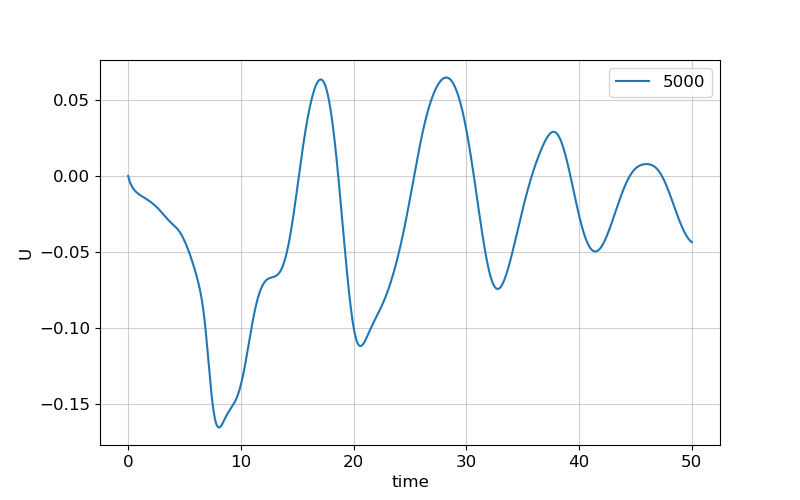
\includegraphics[width = \textwidth]{plots/plot1.png}
    \caption{$U$ in middle of domain for different $Re$-values}
    \label{plot1}
\end{figure}
Clearly the cases with lower Reynold's number converges to a steady flow quicker than the cases with
a higher number. This is due to the amount of turbulance is greater in the case with higher $Re$; 
the intertial forces are greater in comparison to the viscous forces when the $Re$ increases.

Judging by the plot in Figure \ref{plot1} the $Re-25$ case 
\subsection*{Question 5}
Using OpenFoam in each of the cases A-C the following data where obtained: Figure \ref{caseA} shows
both a solution from the Python implementation as well as OpenFOAM solution with the data visualized in matplotlib.

\begin{figure}[H]
    \centering
    \begin{subfigure}[b]{0.475\textwidth}
        \centering
        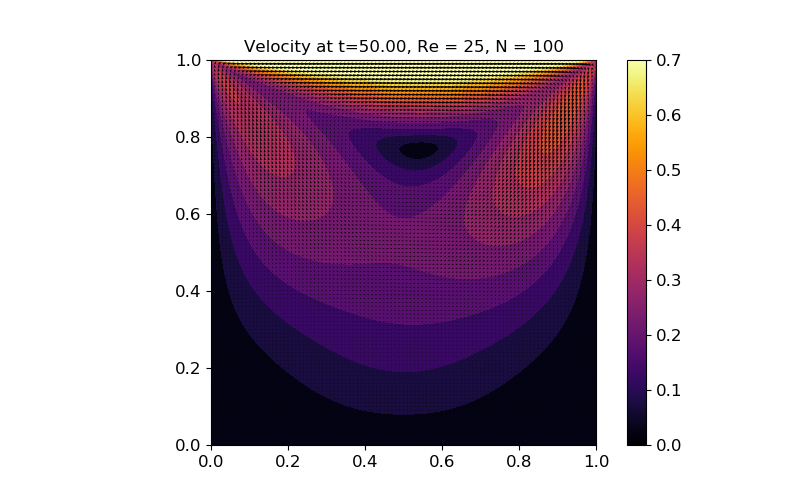
\includegraphics[width=\textwidth]{plots/velocity_RE25_OF.png}
        \caption{OpenFoam solution}
        \label{caseAof}
    \end{subfigure}
    \hfill
    \begin{subfigure}[b]{0.475\textwidth}
        \centering
        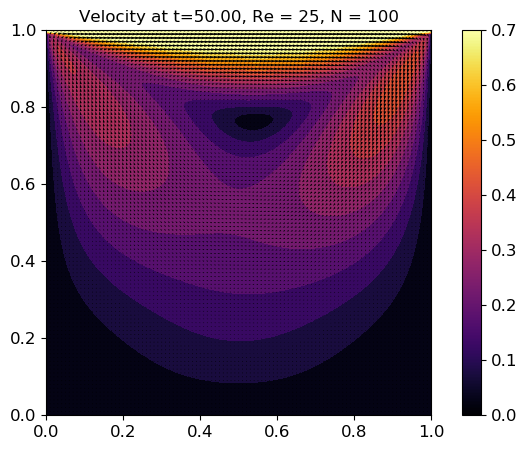
\includegraphics[width=\textwidth]{plots/velocity_RE25.png}
        \caption{Python Solution}
        \label{caseApy}
    \end{subfigure}
    \caption{Case A}
    \label{caseA}
\end{figure}
For a more detailed comparison we can observe the velocity magnitude along the diagonal of the domain,
so called a \textit{plot over line} visualization. For case A we have the following:
\begin{figure}[H]
    \centering
    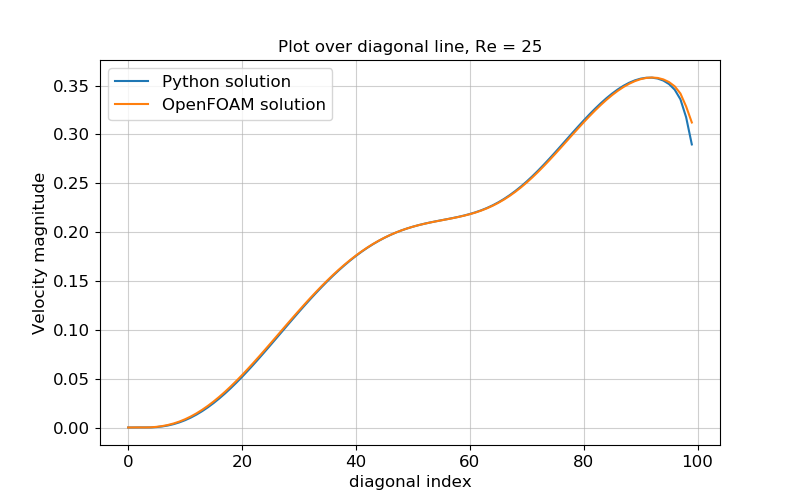
\includegraphics[width = \textwidth]{plots/overline_RE25.png}
    \caption{Plot over line (Case A): Python against OpenFOAM}
\end{figure}
Likewise we can compare case B and C in a similar manner:
\begin{figure}[H]
    \centering
    \begin{subfigure}[b]{0.475\textwidth}
        \centering
        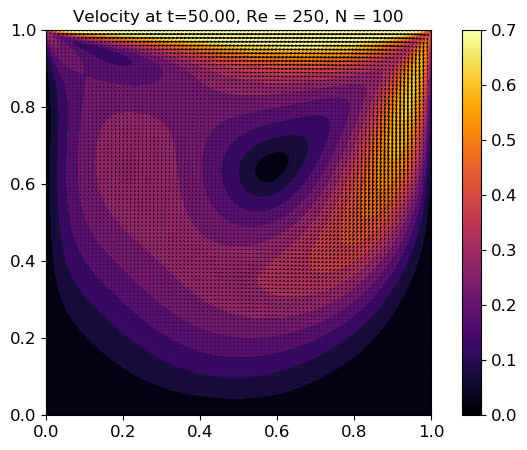
\includegraphics[width=\textwidth]{plots/velocity_RE250_OF.png}
        \caption{OpenFoam solution}
        \label{caseBof}
    \end{subfigure}
    \hfill
    \begin{subfigure}[b]{0.475\textwidth}
        \centering
        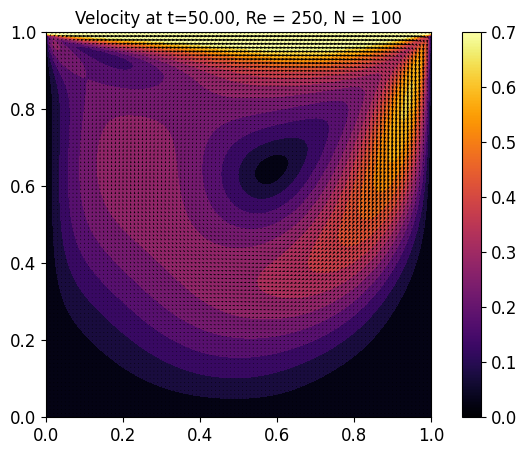
\includegraphics[width=\textwidth]{plots/velocity_RE250.png}
        \caption{Python Solution}
        \label{caseBpy}
    \end{subfigure}
    \caption{Case B}
    \label{caseB}
\end{figure}
\begin{figure}[H]
    \centering
    \begin{subfigure}[b]{0.475\textwidth}
        \centering
        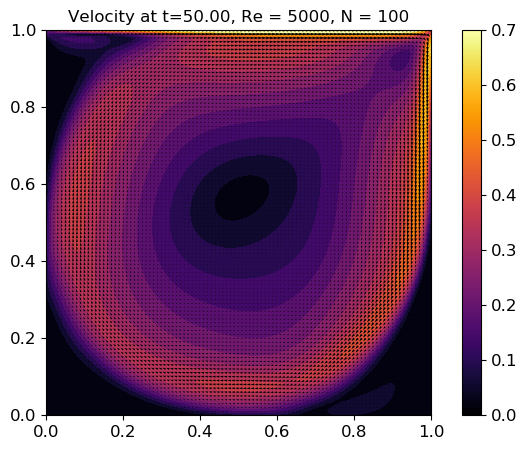
\includegraphics[width=\textwidth]{plots/velocity_RE5000_OF.png}
        \caption{OpenFoam solution}
        \label{caseCof}
    \end{subfigure}
    \hfill
    \begin{subfigure}[b]{0.475\textwidth}
        \centering
        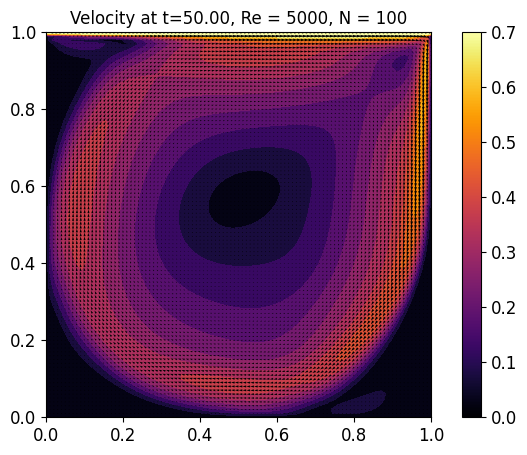
\includegraphics[width=\textwidth]{plots/velocity_RE5000.png}
        \caption{Python Solution}
        \label{caseCpy}
    \end{subfigure}
    \caption{Case C}
    \label{caseC}
\end{figure}
\begin{figure}[H]
    \centering
    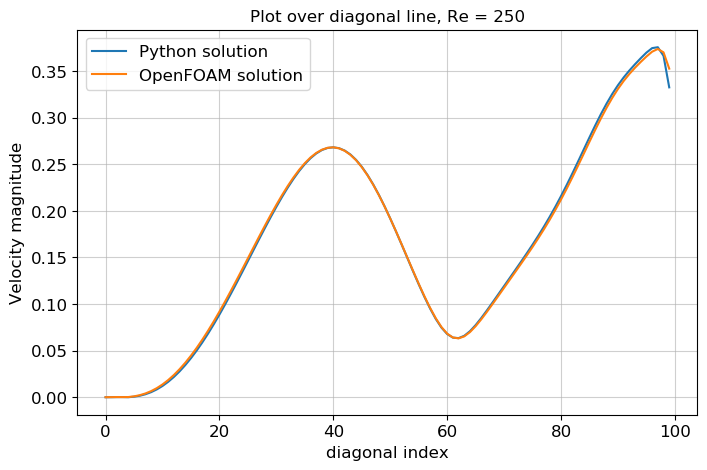
\includegraphics[width = \textwidth]{plots/overline_RE250.png}
    \caption{Plot over line (Case B): Python against OpenFOAM}
\end{figure}
\begin{figure}[H]
    \centering
    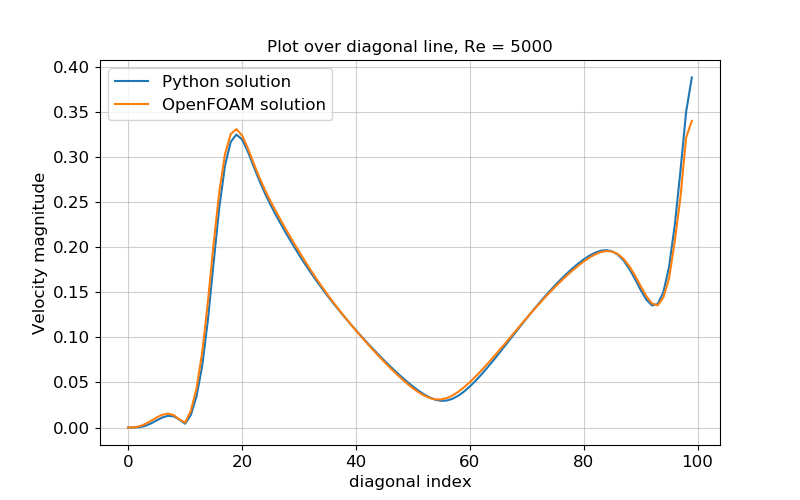
\includegraphics[width = \textwidth]{plots/overline_RE5000.png}
    \caption{Plot over line (Case C): Python against OpenFOAM}
\end{figure}
We can conclude that the Python and OpenFOAM solutions converges, and notably the largest differences was found close to
the boundaries.

Comparing the $L_2$-norm between the different steady solutions we got the following data:
\begin{lstlisting}
    %%INSERT DATA
\end{lstlisting}
\subsection*{Question 6}

\begin{figure}[H]
    \centering
    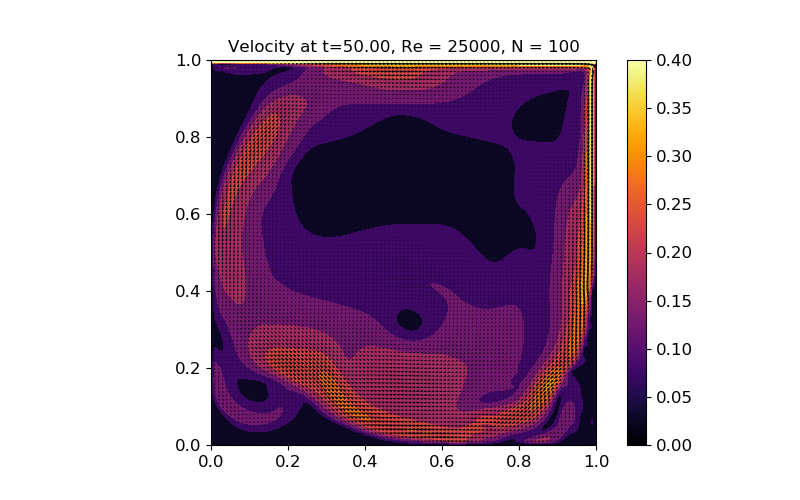
\includegraphics[width = \textwidth]{plots/velocity_D.png}
    \caption{Case D}
    \label{caseD1}
\end{figure}
\begin{figure}[H]
    \centering
    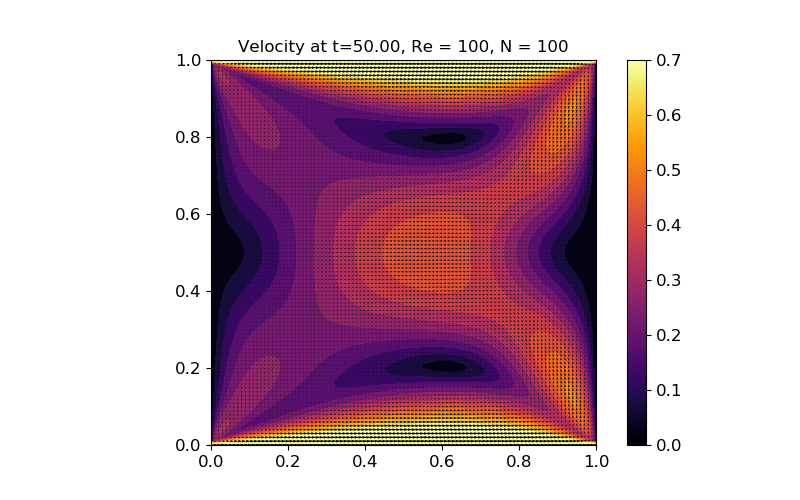
\includegraphics[width = \textwidth]{plots/velocity_D1.png}
    \caption{Bonus case with even higher $Re$}
    \label{caseD}
\end{figure}
\end{document}